% \subfloat[Unstructured data]{%
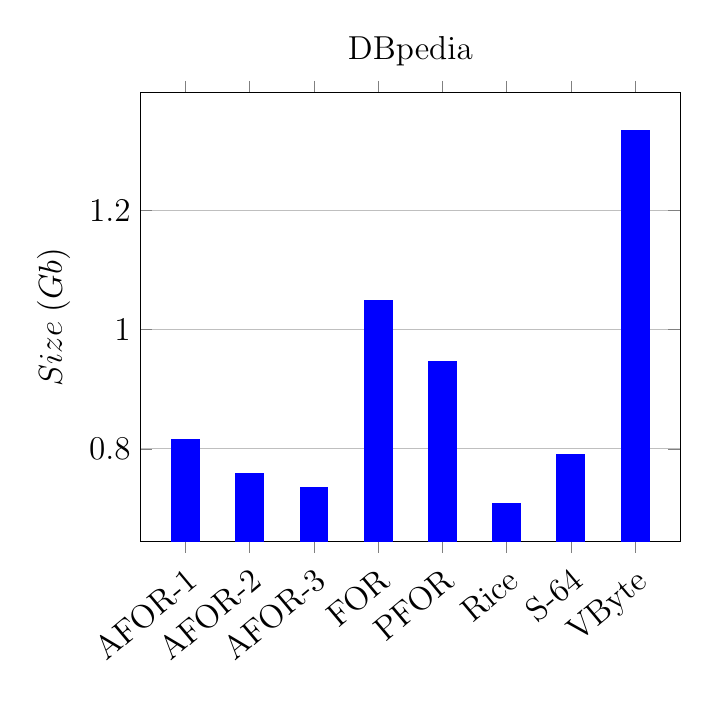
\begin{tikzpicture}[baseline]
\begin{axis}[
ylabel=$Size \; (Gb)$,
x tick label style={rotate=40, anchor=north east},
xtick={1,...,8},
xticklabels={AFOR-1, AFOR-2, AFOR-3, FOR, PFOR, Rice, S-64, VByte},
legend style={at={(0.5,1.13)}, anchor=north, legend columns=-1},
label style={font=\large},
tick label style={font=\large},
title style={font=\large},
ybar,
ymajorgrids=true,
bar width=10pt,
title={DBpedia},
%enlargelimits=0.15,
]
\addplot[draw=blue,fill=blue]
coordinates {(1, 0.816) (2, 0.758) (3, 0.736) (4, 1.049) (5, 0.946) (6, 0.708) (7, 0.791) (8, 1.335)};
\end{axis}
\end{tikzpicture}%
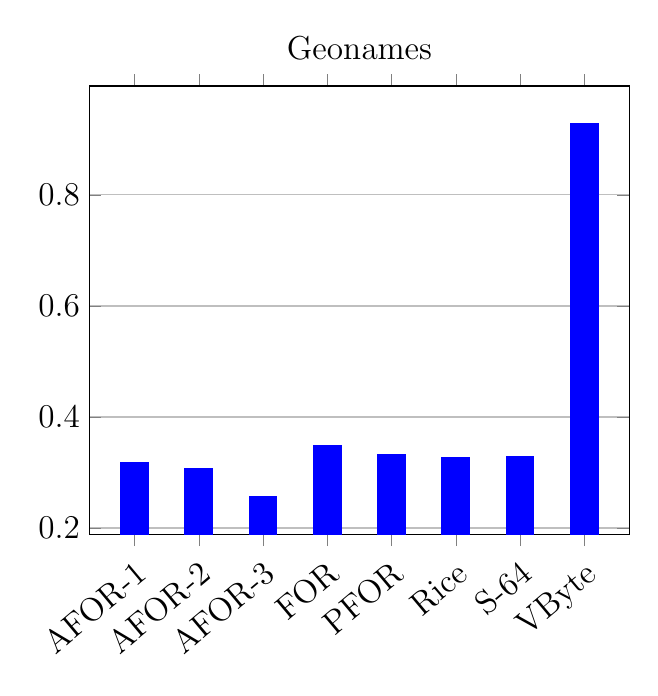
\begin{tikzpicture}[baseline]
\begin{axis}[
x tick label style={rotate=40, anchor=north east},
xtick={1,...,8},
xticklabels={AFOR-1, AFOR-2, AFOR-3, FOR, PFOR, Rice, S-64, VByte},
legend style={at={(0.5,1.13)}, anchor=north, legend columns=-1},
label style={font=\large},
tick label style={font=\large},
title style={font=\large},
ybar,
ymajorgrids=true,
bar width=10pt,
title={Geonames},
%enlargelimits=0.15,
]
\addplot[draw=blue,fill=blue]
coordinates {(1, 0.318) (2, 0.307) (3, 0.256) (4, 0.349) (5, 0.332) (6, 0.327) (7, 0.329) (8, 0.929)};
\end{axis}
\end{tikzpicture}%
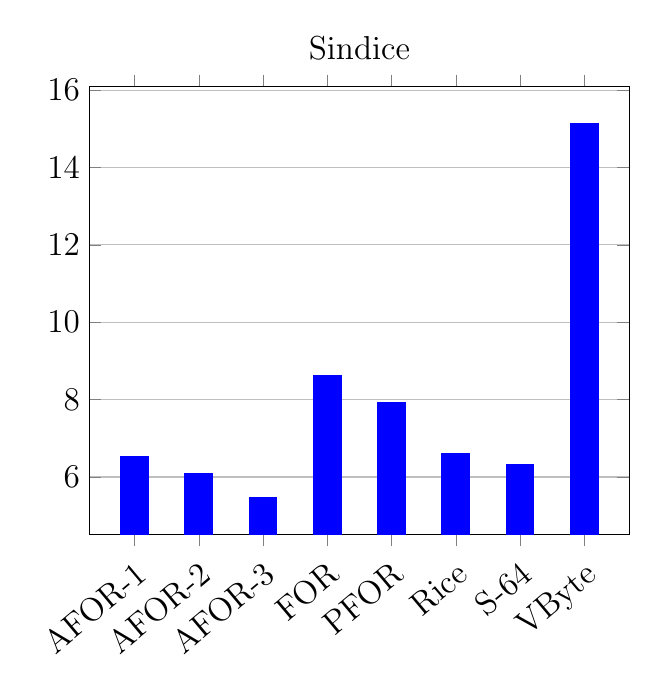
\begin{tikzpicture}[baseline]
\begin{axis}[
x tick label style={rotate=40, anchor=north east},
xtick={1,...,8},
xticklabels={AFOR-1, AFOR-2, AFOR-3, FOR, PFOR, Rice, S-64, VByte},
legend style={at={(0.5,1.13)}, anchor=north, legend columns=-1},
label style={font=\large},
tick label style={font=\large},
title style={font=\large},
ybar,
ymajorgrids=true,
bar width=10pt,
title={Sindice},
%enlargelimits=0.15,
]
\addplot[draw=blue,fill=blue]
coordinates {(1, 6.537) (2, 6.082) (3, 5.475) (4, 8.611) (5, 7.924) (6, 6.605) (7, 6.313) (8, 15.132)};
\end{axis}
\end{tikzpicture}%
% }